
\documentclass[11pt]{beamer}

% contains the complete preamble
\usepackage{present}
\usepackage{custom_underline}
         		               		
\title{}
\author[Felix Z.~Hoffmann]{Felix Z.~Hoffmann}
\institute{}
\date{\today}     


\begin{document}


\begin{frame}{Bordeaux18 talk}

  

  
  
\end{frame}


% pre-Intro: About me - what qualifies me to tell you
% anything about reproducibility/open science. Whom am
% I to talk?

\begin{frame}{Who am I?}
  % 
  \begin{columns}
    %
    \begin{column}{.625\textwidth}
      \minipage[c][0.65\textheight][s]{\columnwidth}

      PhD student with Prof.~Jochen Triesch
      \vspace{0.15cm}
      
\begin{tabular}{|p{0.9\textwidth}}
      \textit{Computational models of structural plasticity}
\end{tabular}	     
  

      \vfill

      Google Summer of Code 2014
      \vspace{0.15cm}

      \begin{tabular}{|p{0.9\textwidth}}
        \textit{Data-centric views in Sumatra}
      \end{tabular}	     

      \vfill

      Wikimedia Open Science Fellow 2017/2018
      \vspace{0.15cm}

      \begin{tabular}{|p{0.9\textwidth}}
        \textit{Open computational research study}
      \end{tabular}	     

      
      
      \endminipage      
    \end{column}
    %
    \begin{column}{.249\textwidth}
      \minipage[c][0.7\textheight][s]{\columnwidth}

      \begin{figure}
        \centering
        \includegraphics[width=\textwidth]{%
          logo_fias+mpi.png} %
      \end{figure}
      
      \begin{figure}
        \centering
        \includegraphics[width=\textwidth]{%
          logo_gsoc14.jpg} %
      \end{figure}

      \begin{figure}
        \centering
        \includegraphics[width=\textwidth]{%
          logo_wosf.png} %
      \end{figure}
      \endminipage      

      
      
    \end{column}
  \end{columns}
  %  
\end{frame}



% Intro: Why we (might) need to do things differently
% from our supervisors/how it's been done until now
\begin{frame}{The reproducibility crisis}

  \begin{figure}
    \centering
    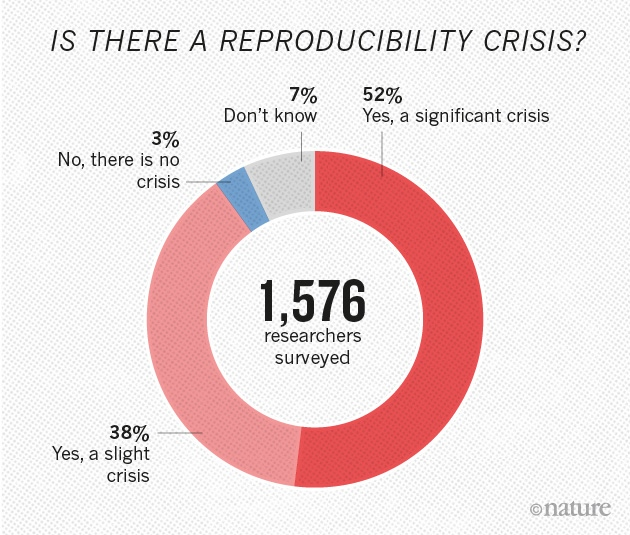
\includegraphics[width=0.85\textwidth]{%
    img/reproducibility_crisis_q.jpeg} %
  \end{figure}
  

  
  
\end{frame}


% So what can we do? -> A call for open source in
% neuroscience
\begin{frame}{Open Source for Neuroscience}

  \begin{figure}
    \centering
    \includegraphics<1>[width=0.9\textwidth]{%
      img/open_source_neuroscience.png} %
    \includegraphics<2>[width=0.9\textwidth]{%
      img/pledge.png} %
    \includegraphics<3>[width=0.9\textwidth]{%
      img/pledge_underline.png} %
  \end{figure}

  \onslide<2->
  \begin{center}
    \href{http://opensourceforneuroscience.org/}{opensourceforneuroscience.org/}
  \end{center}
  

  
  
\end{frame}


% But what does this mean? Does open == reproducible?
% What do we need to do to make our code reproducible?
% --> Rougier's five Rs
\include{frames/what_open_and_reproducible_means}

% Does it really work? Yes! I think. Here's an example
% how things can be done --> My project


\begin{frame}{Wikimedia Open Science Fellowship}

  %% - picture of the current fellows
  \begin{figure}
    \centering
    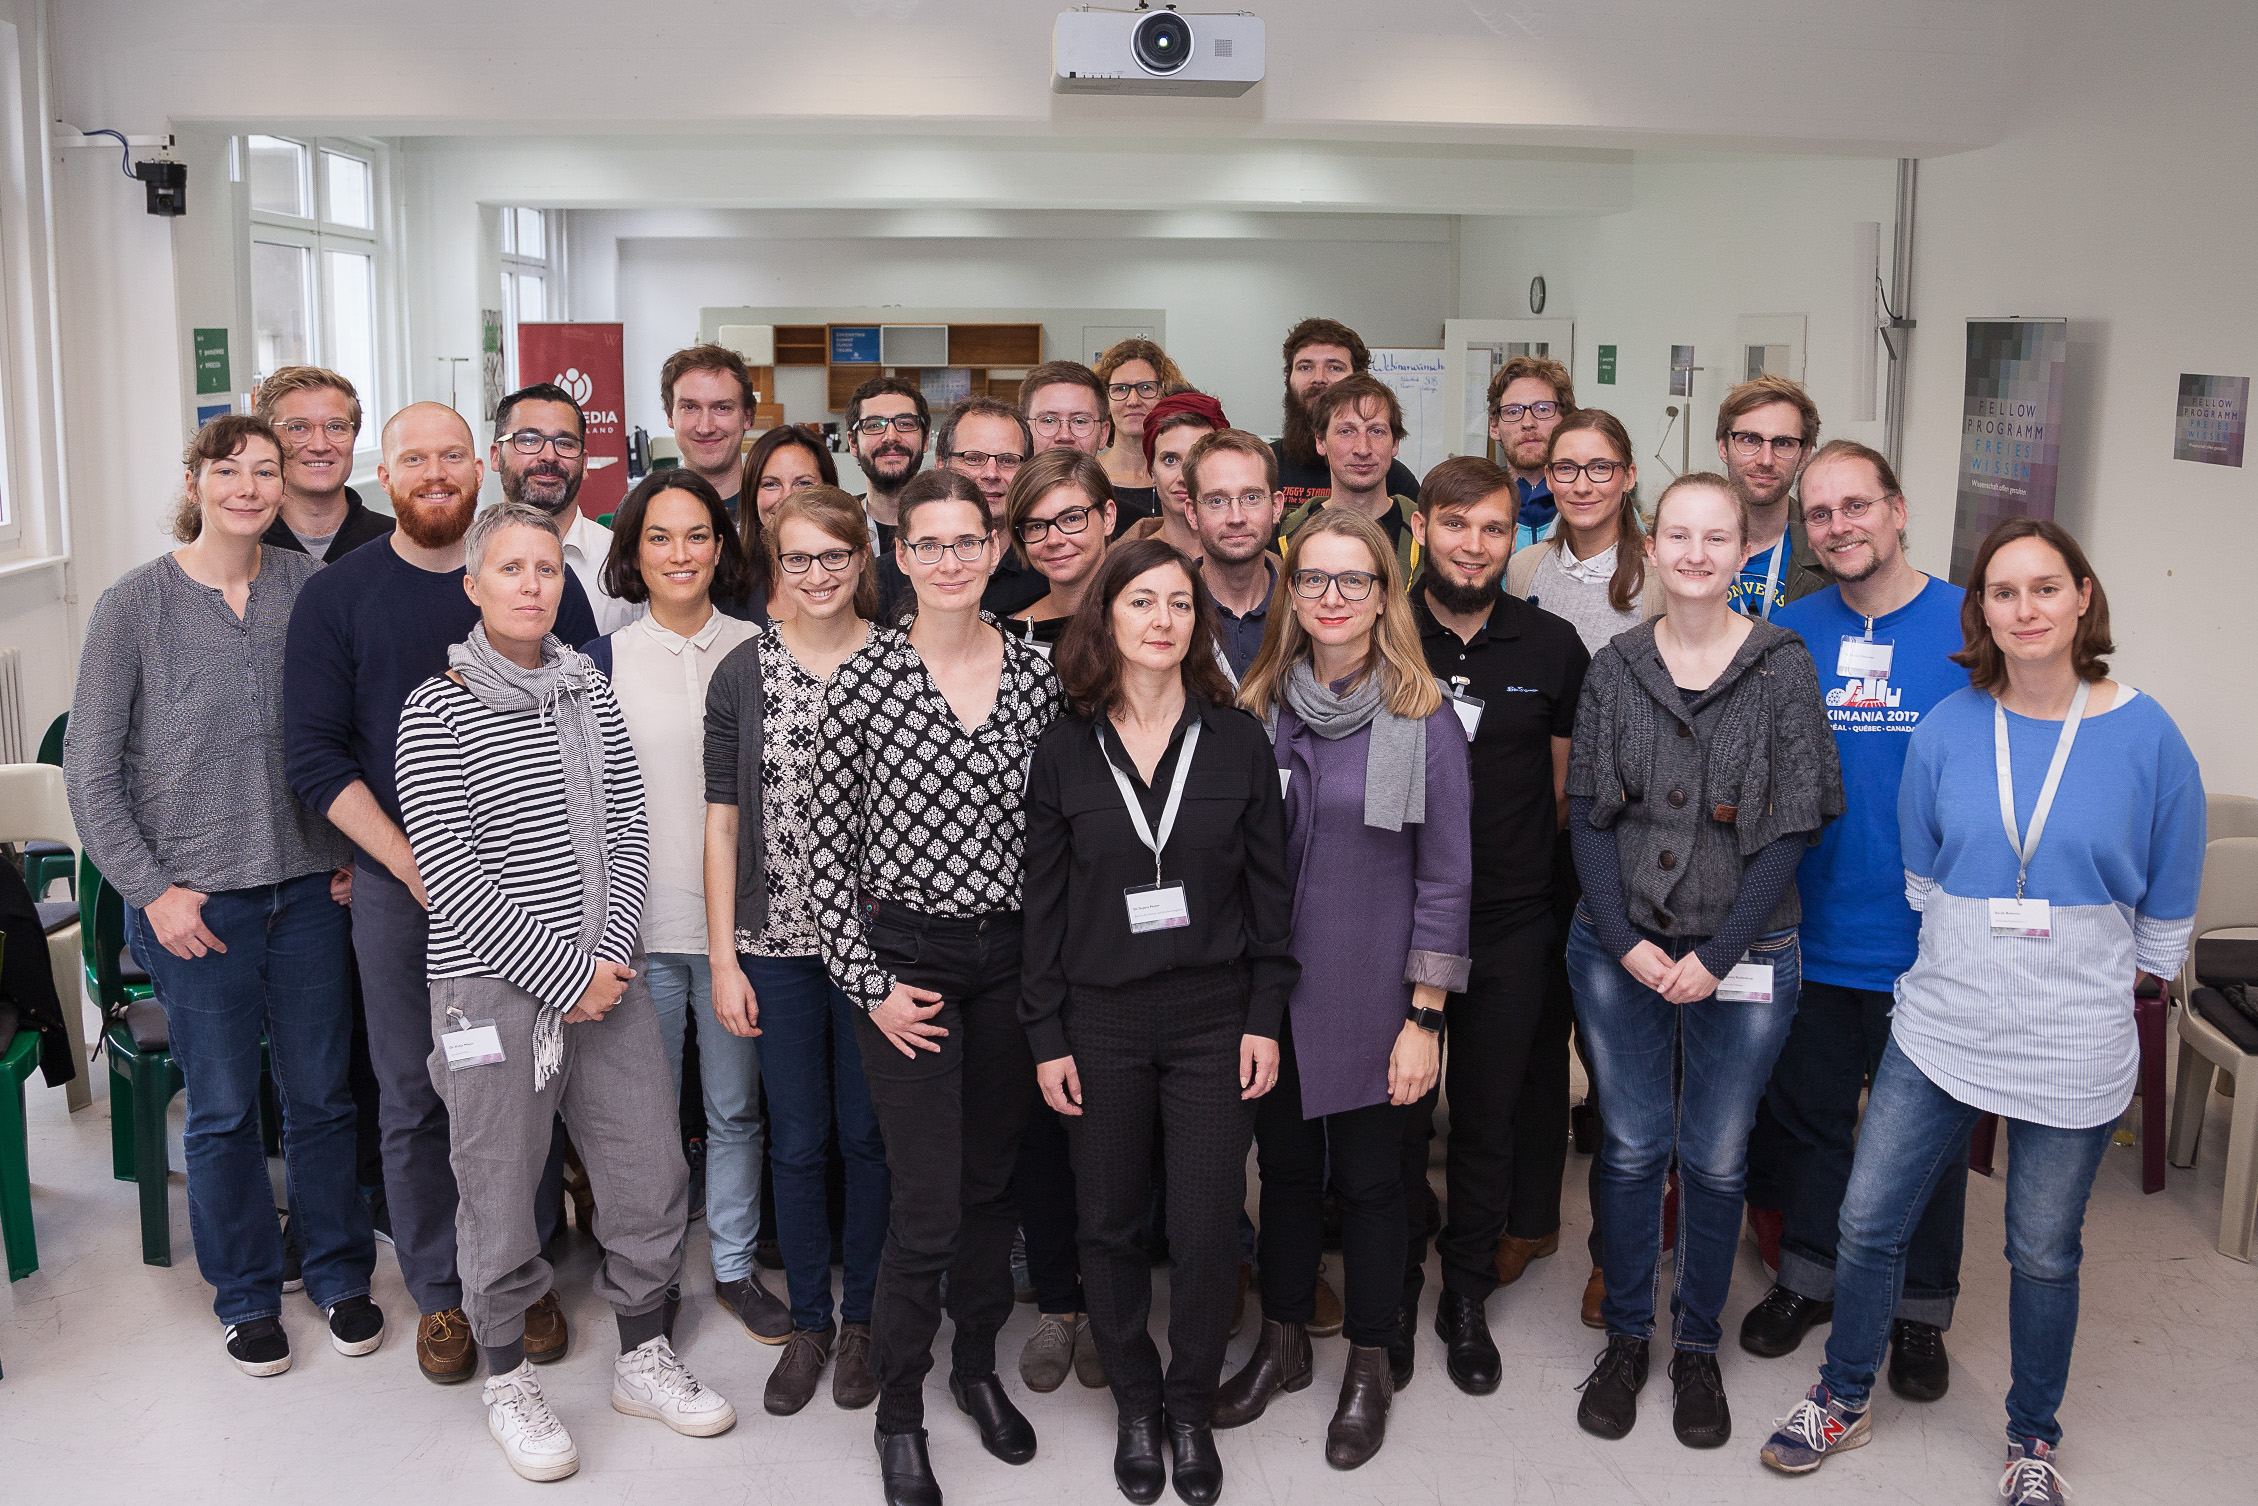
\includegraphics[width=0.875\textwidth]{%
    img/WOSF2017.jpg} %
  \end{figure}
  

  \source{\tiny Photo: Ralf Rebmann, CC BY-SA 4.0}


\end{frame}




\begin{frame}{Wikimedia Open Science Fellowship}

  % 
  \begin{columns}
    %
    \begin{column}{.55\textwidth}


      \begin{figure}
        \centering
        
\includegraphics[width=0.96\textwidth]{%
        img/logo_wosf_full.png} %
      \end{figure}
      

      
      

    \end{column}
    %
    \begin{column}{.45\textwidth}
      \minipage[c][0.625\textheight][s]{\columnwidth}

      \vspace{0.2cm}
      
      \begin{itemize}[leftmargin=*]

      \item[-] runs from October to June

      \item[-] fellows are paired with a mentor who supports the progress

      \item[-] financial support offered

      \item[-] program in German

      \item[-]       application for 3rd round now open!
      \href{http://bit.ly/osfprog}{bit.ly/osfprog}


      \end{itemize}

      

      \endminipage      
    \end{column}
  \end{columns}
  
\end{frame}




% So what can I take out of this talk? Give some rules
% and guide lines to follow (other resources)?

\begin{frame}{}

  - Zenodo
  - Open Science Framework
  -  
  
\end{frame}



\begin{frame}[t]{References \hspace{3.25cm} }

  \begin{multicols}{2}
    \printbibliography
  \end{multicols}
  \vspace{0.25cm}
  \begin{center}
    \LARGE
    \textit{Thank you!}
  \end{center}

  \pnote {

  }
  
\end{frame}




\end{document}
















